\documentclass{article}

\usepackage[margin=1in]{geometry}
\usepackage{fancyhdr}
\usepackage{amsmath}
\usepackage{amssymb}
\usepackage{listings}
\usepackage{graphicx}
\usepackage{enumerate}
\usepackage{tikz}
\usetikzlibrary{automata,positioning}


\pagestyle{fancy}

\lhead{CS 373 \\ Homework 2}
\chead{}
\rhead{Drew Cross (ddcross2)\\
    \emph{Partners:} Eric Parsons}
\lfoot{}
\cfoot{}
\rfoot{}

\begin{document}

\section*{Homework 2}

\subsection*{Problem 1}

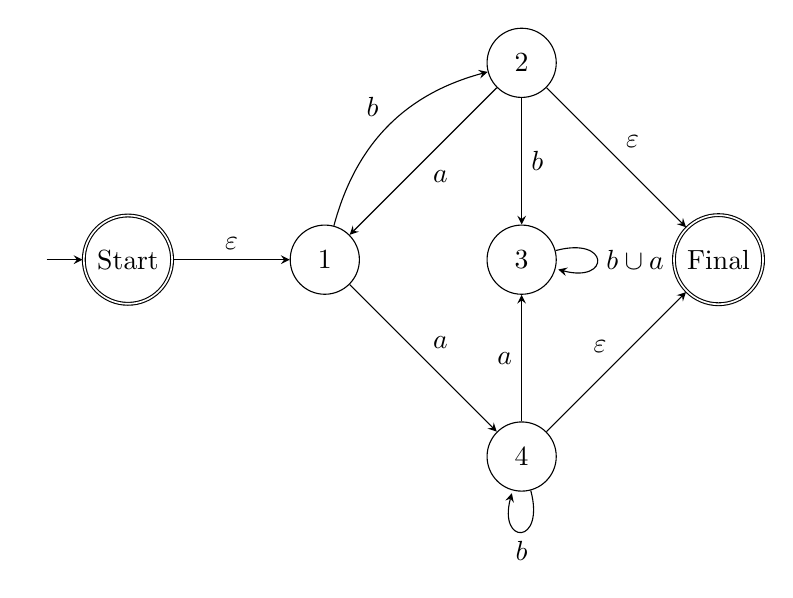
\begin{tikzpicture}[%
>=stealth,
node distance=2.5cm,
on grid,
auto
]

\node[initial,initial text=,state,accepting] (0)  {Start};
\node[state] (1) [right of=0] {1};
\node[state] (3) [right of=1] {3};
\node[state] (2) [above of=3] {2};
\node[state] (4) [below of=3] {4};
\node[state, accepting] (5) [right of=3] {Final};

\path[->] (0) edge node {$\varepsilon$} (1);
\path[->] (1) edge[bend left] node {$b$} (2);
\path[->] (2) edge node {$a$} (1);
\path[->] (2) edge node {$\varepsilon$} (5);
\path[->] (2) edge node {$b$} (3);
\path[->] (1) edge node {$a$} (4);
\path[->] (3) edge[loop right] node {$b \cup a$} (3);
\path[->] (4) edge[loop below] node {$b$} (4);
\path[->] (4) edge node {$\varepsilon$} (5);
\path[->] (4) edge node {$a$} (3);

\end{tikzpicture}
\\[5pt]

%%%%%%%%%%%% Part 2 of problem 1 %%%%%%%%%%%%%%%%%
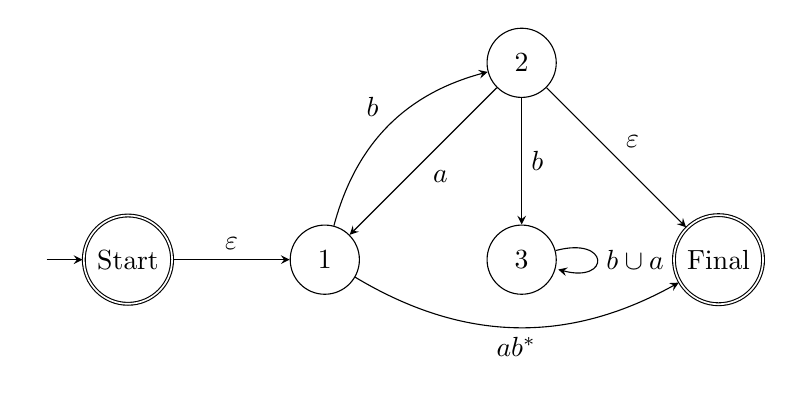
\begin{tikzpicture}[%
>=stealth,
node distance=2.5cm,
on grid,
auto
]

\node[initial,initial text=,state,accepting] (0)  {Start};
\node[state] (1) [right of=0] {1};
\node[state] (3) [right of=1] {3};
\node[state] (2) [above of=3] {2};
\node[state, accepting] (5) [right of=3] {Final};

\path[->] (0) edge node {$\varepsilon$} (1);
\path[->] (1) edge[bend left] node {$b$} (2);
\path[<-] (5) edge[bend left] node {$ab^*$} (1);
\path[->] (2) edge node {$a$} (1);
\path[->] (2) edge node {$\varepsilon$} (5);
\path[->] (2) edge node {$b$} (3);
\path[->] (3) edge[loop right] node {$b \cup a$} (3);

\end{tikzpicture}
\\[5pt]

%%%%%%%%%%%% Part 3 of problem 1 %%%%%%%%%%%%%%%%%
\begin{tikzpicture}[%
>=stealth,
node distance=2.5cm,
on grid,
auto
]

\node[initial,initial text=,state,accepting] (0)  {Start};
\node[state] (1) [right of=0] {1};
\node[state, yshift=-2em] (2) [above of=3] {2};
\node[state, accepting] (5) [right of=3] {Final};

\path[->] (0) edge node {$\varepsilon$} (1);
\path[->] (1) edge[bend  left] node {$b$} (2);
\path[->] (1) edge node {$ab^*$} (5);
\path[->] (2) edge node {$a$} (1);
\path[->] (2) edge node {$\varepsilon$} (5);

\end{tikzpicture}
\\[5pt]

%%%%%%%%%%%% Part 4 of problem 1 %%%%%%%%%%%%%%%%%
\begin{tikzpicture}[%
>=stealth,
node distance=2.5cm,
on grid,
auto
]

\node[initial,initial text=,state,accepting] (0)  {Start};
\node[state] (1) [right of=0] {1};
\node[state, accepting] (5) [right of=3] {Final};

\path[->] (0) edge node {$\varepsilon$} (1);
\path[->] (1) edge[loop above] node {$ba$} (1);
\path[->] (1) edge node {$ab^*$} (5);

\end{tikzpicture}
\\[5pt]

%%%%%%%%%%%% Part 5 of problem 1 %%%%%%%%%%%%%%%%%
\begin{tikzpicture}[%
>=stealth,
node distance=2.5cm,
on grid,
auto
]

\node[initial,initial text=,state,accepting] (0)  {Start};
\node[state, accepting] (5) [right of=3] {Final};

\path[->] (0) edge node {$(ba)^* \cup b \cup ab^*$} (5);

\end{tikzpicture}

\newpage

%%%%%%%%%%%%%%%%%%%%%%%PAGE%%%%%%%%%%%%%%%%%%%%%%%%%%
\section*{Homework 2}

\subsection*{Problem 2}

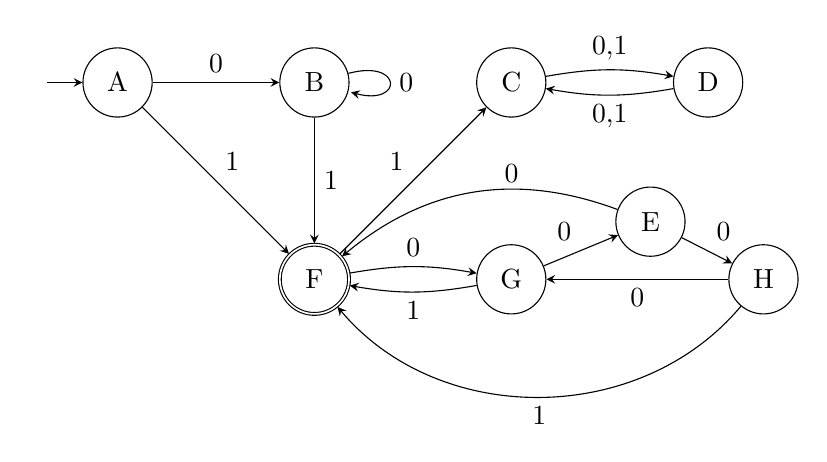
\begin{tikzpicture}[%
>=stealth,
node distance=2.5cm,
on grid,
auto
]

\node[initial,initial text=,state] (0)  {A};
\node[state] (1) [right of=0] {B};
\node[state] (2) [right of=1] {C};
\node[state] (3) [right of=2] {D};
\node[state] (4) [below right of=2] {E};
\node[state, accepting] (5) [below of=1] {F};
\node[state] (6) [right of=5] {G};
\node[state, xshift=2em] (7) [right of = 6] {H};

\path[->] (0) edge node {0} (1);
\path[->] (0) edge node {1} (5);
\path[->] (1) edge[loop right] node {0} (1);
\path[->] (1) edge node {1} (5);
\path[->] (2) edge[bend left=10] node {0,1} (3);
\path[->] (3) edge[bend left=10] node {0,1} (2);

\path[->] (5) edge node {1} (2);
\path[->] (5) edge[bend left=10] node {0} (6);
\path[->] (6) edge[bend left=10] node {1} (5);
\path[->] (6) edge node {0} (4);
\path[->] (7) edge node {0} (6);
\path[->] (7) edge[bend left=50] node {1} (5);

\path[->] (4) edge node {0} (7);
\path[<-] (5) edge[bend left] node[xshift=2em] {0} (4);

\end{tikzpicture}
\\[10pt]

\begin{tabular}{r|c|c|c|c|c|c|c|}
\hline
 &A&B&C&D&E&F&G\\
\hline
B& &-&-&-&-&-&-\\
\hline
C&x&x&-&-&-&-&-\\
\hline
D&x&x& &-&-&-&-\\
\hline
E& & &x&x&-&-&-\\
\hline
F&x&x&x&x&x&-&-\\
\hline
G& & &x&x& &x&-\\
\hline
H& & &x&x& &x& \\
\hline
\end{tabular}
\\[10pt]

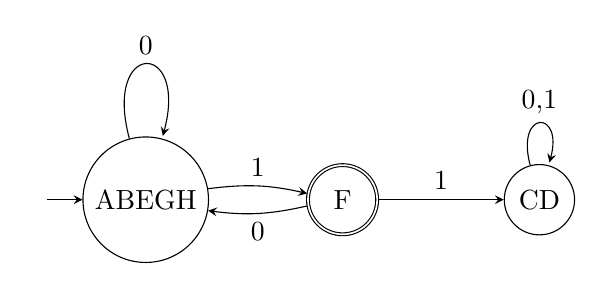
\begin{tikzpicture}[%
>=stealth,
node distance=2.5cm,
on grid,
auto
]

\node[initial,initial text=,state] (0)  {ABEGH};
\node[state, accepting] (1) [right of=0] {F};
\node[state] (2) [right of=1] {CD};

\path[->] (0) edge[loop above] node {0} (0);
\path[->] (0) edge[bend left=10] node {1} (1);
\path[->] (1) edge[bend left=10] node {0} (0);
\path[->] (1) edge node {1} (2);
\path[->] (2) edge[loop above] node {0,1} (2);

\end{tikzpicture}

\newpage
\section*{Homework 2}

\subsection*{Problem 3}
\begin{enumerate}[a)]
        \item Let:
    \[ E = \{ w \in \Sigma^* ~|~ \text{$w$ does not contain substring $\$\$\$ $ and } \#\$(w) = \#1(w) + \#2(w) + \#2(w) \} \]
    We use the pumping lemma to prove that $E$ is not regular.
    This proof is by contradiction.\\
    Assume $E$ is regular. Let $p$ be the pumping length given by the pumping lemma. \\
    Choose $s$ to be the string $1^p(\$\$1)^p$. \\
    Because $s$ is a member of $E$ and $s$ has more length than $p$,
    the pumping lemma guarantees that $s$ can be split into three pieces,
    $s = xy^iz$, where for any $i \geq 0$ the string $xy^iz$ is in $E$. \\
    Since the string must start with $p$ number of $1$'s $|xy| > p$. Then $xy$ must lie in
    the first part $(1^p)$. When $s = xyyz$ we end up with $1^{p+1}(\$\$1)^p$ and we now
    have more $1$'s than $\$$'s, and
    we have found a contradiction, $E$ cannot be regular.
    \[ \square \]

    \item Let: \\
    \[ E = \{ w \in \Sigma^* ~|~ \text{$w$ does not contain substring $\$\$\$ $ and } \#\$(w) = \#1(w) + \#2(w) + \#2(w) \} \]
    We use closure over regular languages to prove that $E$ is not regular.
    This proof is by contradiction.\\
    First: $ E \cap \{ (\$\$1)^p1^p | p \geq 1 \} $ \\
    Define the inverse homomorphism $h^{-1}(\$\$1) \rightarrow 0$ \\
    Now we have: $\{0^p1^p | p \geq 1 \}$ \\
    Now take $\{ 0^p1^p | p \geq 1 \} \cup \varepsilon $ \\
    And we are left with: $\{ 0^p1^p | p \geq 0 \} $ \\
    and we know that $ \{ 0^n1^n | n \geq 0\} $ is not regular. \\
    But since we assumed $E$ was regular and we used operations that were closed
    under regular languages we have found that $E$ is not regular.
    \[ \square \]

\end{enumerate}

\newpage
\section*{Homework 2}

\subsection*{Problem 4}
\begin{enumerate}[a)]
    \item Let: \[A = \{xyx^R ~|~ x \in \Sigma, y \in \Sigma^*\}\]
        Claim: $A$ is regular: \\
        Proof: \\

        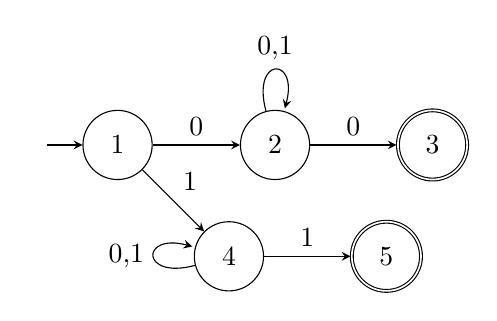
\begin{tikzpicture}[%
        >=stealth,
        node distance=2cm,
        on grid,
        auto
        ]

        \node[initial,initial text=,state] (1)  {1};
        \node[state] (2) [right of=1] {2};
        \node[state, accepting] (3) [right of=2] {3};
        \node[state] (4) [below right of=1] {4};
        \node[state, accepting] (5) [right of=4] {5};

        \path[->] (1) edge node {0} (2);
        \path[->] (2) edge[loop above] node {0,1} (2);
        \path[->] (2) edge node {0} (3);
        \path[->] (1) edge node {1} (4);
        \path[->] (4) edge node {1} (5);
        \path[->] (4) edge[loop left] node {0,1} (4);

        \end{tikzpicture}

    Explanation:
    Since $x$ is a single symbol, the fact that it is reversed is irrelevant as this collapses
    down to $xyx$. So we can write a DFA that represents that language.
    \[\square\]

    \item Let: \[B = \{xyx^R ~|~ x \in \Sigma^*, y \in \Sigma\}\]
    We use the pumping lemma to prove that $B$ is not regular.
    This proof is by contradiction.\\
    Assume $B$ is regular. Let $p$ be the pumping length given by the pumping lemma. \\
    Choose $s$ to be the string $1^p01^p$, which is in $B$. \\
    Because $s$ is a member of $B$ and $s$ has more length than $p$,
    the pumping lemma guarantees that $s$ can be split into three pieces,
    $s = xy^iz$, where for any $i \geq 0$ the string $xy^iz$ is in $B$. \\
    In this case $x$ and $y$ must be in the first $1^p$ by condition 3 of the pumping lemma.
    When $s = xyyz$ we have $1^{p+1}01^p$ but this is not in the original language.
    \[\square\]

    \item Let: \[C = \{xyx^R ~|~ x \in \Sigma^*, y \in \Sigma^*\}\]
        Claim: $C$ is regular: \\
        Proof:

        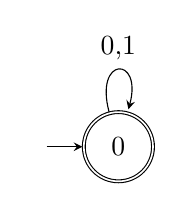
\begin{tikzpicture}[%
        >=stealth,
        node distance=2.5cm,
        on grid,
        auto
        ]

        \node[initial,initial text=,state,accepting] (0)  {0};

        \path[->] (0) edge[loop above] node {0,1} (0);

        \end{tikzpicture}

    Explanation:\\
    If we let $x = \varepsilon$ then we are left with $y$, but $y \in \Sigma^*$ so 
    $C = \{xyx^R ~|~ x \in \Sigma^*, y \in \Sigma^*\}$
    is just another way to write $\Sigma^*$
    \[\square\]

    \item $D = \{xyy^Rx^R ~|~ x \in \Sigma^*, y \in \Sigma^*\}$\\
    Observe that $xyy^Rx^R = xy(xy)^R.$ \\
    Define a homomorphism $h(z)=xy$ so: $h^{-1}(xy) = z$.\\
    Then $h$ maps $D$ to a new language $D' = \{zz^R\ | z \in \Sigma^*\}$

    We use the pumping lemma to prove that $D'$ is not regular and thus $D$ is not regular.
    This proof is by contradiction.\\
    Assume $D'$ is regular. Let $p$ be the pumping length given by the pumping lemma. \\
    Now pick $s$ to be $0^p110^p$ which is in $D'$.\\
    Because $s$ is a member of $D'$ and $s$ has more length than $p$,
    the pumping lemma guarantees that $s$ can be split into three pieces,
    $s = xy^iz$, where for any $i \geq 0$ the string $xy^iz$ is in $D'$. \\
    By condition 3 of the pumping lemma $x$ and $y$ must lie within the first $0$ of the
    string. Otherwise $|xy| > p$. But when $s=xyyz$ our string is $0^{p+1}110^p$ which
    is not in the language defined above. So we have a contradiction.
    \[\square\]
\end{enumerate}

\newpage
\section*{Homework 2}

\subsection*{Problem 5}
\begin{enumerate}[a)]

    \item For any regular expression $R$, if $L(R)$ is infinite,
    then $R$ contains a Kleene star.\\
    Proof:\\
    There are only 3 operations for regular expressions, union, concatenation and the star.
    To prove this we consider the following cases:
    \begin{enumerate}[1)]
    \item If you have two finite languages $A$ and $B$ when you take the union of $A$ and $B$
    the cardinality of the set is at most $|a| + |b|$.
    \item If you have two finite languages $A$ and $B$ when you take the concatenation
    of $A$ and $B$
    the cardinality of the set is at most $|a| * |b|$.
    \item If you have two finite languages $A$ and $B$ when you take the Kleene star of
    $A$ and $B$ you are left with strings of infinite length by the definition of the
    Kleene star.
    \end{enumerate}

    Therefore the only operation on regular expressions that yields infinite length strings
    is the Kleene star.
    \item For any regular expression $R$, if $R$ contains a Kleene star,
    then $L(R)$ is infinite. \\
    Disproof:
    If we concatenate $\varnothing$ with the Kleene star we are left with $\varnothing$.
    Formally,
    $\Sigma^* \circ \varnothing$

    \item The regular expression symbol $\varnothing$ is needed only to
    describe the regular language $\varnothing$.
    That is, for any regular expression $R$ containing a $\varnothing$,
    there is an alternate expression $R'$ with $L(R) = L(R')$ such that $R'$
    does not contain a $\varnothing$ if and only if $L(R) \neq \varnothing$.

    Proof: \\
    Consider the three types of operations allowed on regular languages:
    \begin{enumerate}[1)]
    \item Concatenation: When $\varnothing$ is concatenated with a regular expression,
    we can remove all regular expressions the empty set is concatenated with and we will
    be left with the same language.
    \item Union: When $\varnothing$ is unioned with other regular expressions we can
    simply drop the $\varnothing$ and everything it is concatenated to by rule 1 above.
    \item Kleene star: When the $\varnothing$ is starred we can replace $\varnothing^*$ with
    $\varepsilon$ because $\varnothing^* = \varepsilon$ by definition.
    \end{enumerate}
    For example: \\
    The regular expression: $\varnothing a \cup \varnothing^* \cup b \cup ab$ \\
    Reduces to: $\varepsilon \cup b \cup ab$

    \end{enumerate}

    \newpage
    \section*{Homework 2}

    \subsection*{Problem 6}

    \begin{enumerate}[a)]
    \item Let a DFA $ M = (Q, \Sigma, \delta, q_0, F)$\\
    Where: \\
    $Q = \{1,\ 2,\ ...\ m-1\}$ \\
    $\Sigma = \{0,\ 1,\ ...\ k-1\}$ \\
    $\delta(a, q) = (q * k + a)\ \%\ m$ where $q$ is the label of the current state. \\
    $q_0 = 0$ \\
    $F = 0$

    This is essentially a generic DFA similar to the one created in lecture that was used
    to tell congruence mod 5 when you have a binary number (1-26-2012).
    In this case the DFA needs to tell you what your remainder is with respect to the
    multiple, $m$, and you only have $k$ numbers to use for transitions. Your $Q$ will
    represent the remainder after performing the operation $(q*k + a) \slash m$\\[5pt]

    Example:

    Consider $n = 2$ and $k = 3$ can be represented by:

    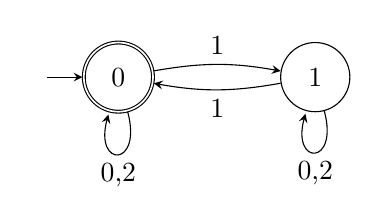
\begin{tikzpicture}[%
    >=stealth,
    node distance=2.5cm,
    on grid,
    auto
    ]

    \node[initial,initial text=,state,accepting] (0)  {0};
    \node[state] (1) [right of=0] {1};

    \path[->] (0) edge[loop below] node {0,2} (0);
    \path[->] (0) edge[bend left=10] node {1} (1);
    \path[->] (1) edge[bend left=10] node {1} (0);
    \path[->] (1) edge[loop below] node {0,2} (1);

    \end{tikzpicture}

    \item Give an example of a $3$-regular set that is not $2$-regular, and prove it.\\

    Attempted proof:
    $2^n(2^n)^R$ in base 3 is regular, because you can draw a DFA which accepts on strings
    that only contain twos. But when you convert $2^n(2^n)^R$ to base 2 you get strings
    that have at least one $1$ and all the strings end in $0$ because you're multiplying
    by an even number $2$ and then adding the last $2$. This will cause the language
    to not be regular because you will need to keep track of all the $1$'s and $0$'s for a
    given n. For example: \\
    $2 = 10$ \\
    $22 = 1000$ \\
    $222 = 11010$ \\
    Since these strings follow no particular pattern I would argue that they are irregular
    but in order to prove this I would need to pump every possible language.


\item Prove that the set of all primes is not $k$-regular for any $k \in \mathbb{N}$. (Hint: You may use the fact that for any integer $x$ and prime $p$, $x^p - x$ is divisible by $p$.) \\
My intuiton here is the same as for part b where the primes have no particular pattern, so they cannot be regular.
But again, I was not able to find a good technique to proving this.

 \end{enumerate}


 \newpage
 \section*{Homework 2}

 \subsection*{Problem 7}
 The problem with the given proof is that with the given $w$ you can pump it. Additionally
 only one substring is given for $y$, when there are multiple cases. For example,
 Let $y = 0^k1^k$, which is acceptable because the proof has selected $k =
 \lfloor\frac{p}{2}\rfloor$. In this case we can pump $y$. \\[5pt]
 Correct Proof (Taken from Sipster pp. 80):
  Let:
  \[ A = \{uv \in \{0,1\}^* ~:~ |u| = |v|, \#0(u) = \#1(v), \text{ and } \#0(v) = \#1(u) \}\]
  We use the pumping lemma to prove that $A$ is not regular.
  This proof is by contradiction.\\
   Assume $A$ is regular. Let $p$ be the pumping length given by the pumping lemma. \\
   Choose $s$ to be the string $1^p0^p$, which is in $A$. \\
   Because $s$ is a member of $A$ and $s$ has more length than $p$,
  the pumping lemma guarantees that $s$ can be split into three pieces,
  $s = xy^iz$, where for any $i \geq 0$ the string $xy^iz$ is in $A$. \\
       Consider these three cases to show that this result is impossible:

       \begin{enumerate}[1)]
       \item The string $y$ consists only of $0$'s. In this case the string $xyyz$ has more
       $0$'s than $1$'s and is not a valid member of $A$. This case is a contradiction.
       \item The string $y$ consists only $1$'s. This case is similar to case 1 and also gives
       a contradiction.
       \item The string $y$ has both $0$'s and $1$'s. In this case the string $xyyz$ may have
       the same number of $0$'s and $1$'s, but they will be out of order with some $1$'s before
       some $0$'s. Hence is not a member of $A$, which is a contradiction.
       \end{enumerate}

       This contradiction is unavoidable if we make the assumption that $B$ is regular, so be is
       not regular.
       \[\square\]

       \end{document}
